\documentclass[11pt]{article}
\usepackage{tikz}
\usetikzlibrary{decorations.pathreplacing,calligraphy}
\usetikzlibrary{calc}
\usetikzlibrary{shapes.geometric}
\usetikzlibrary{arrows.meta}
\usepackage[utf8]{inputenc}
\usepackage[T1]{fontenc}
\usepackage{textcomp,amssymb,amsmath,amsthm}
\usepackage{xcolor}
\tikzset{sttriangle/.style={
    draw=black,
    fill=white,
    regular polygon,
    regular polygon sides=3,
    minimum size = 0pt,
    inner sep=1pt
}}
\tikzset{stcircle/.style={
    fill=white,
    draw=black,
    circle,inner sep=1pt,
    minimum size = 1.5em
}}
\tikzset{rednode/.style={
    fill=white,
    draw=black,
    circle,
    inner sep=1pt,
    minimum size = 1.5em
}}
\tikzset{blacknode/.style={
    text=white,
    fill=black,
    draw=black,
    circle,
    inner sep=1pt,
    minimum size = 0.5em
}}
\tikzset{splitter/.style={
    fill=black,
    circle,
    inner sep=0pt,
    minimum size = 4pt
}}
\tikzset{term/.style={
    draw=black,
    fill=black,
    rectangle,
    inner sep=0pt,
    minimum size=4pt
}}
\tikzset{chooser/.style={
    draw=black,
    fill=white,
    circle,
    inner sep=0pt,
    minimum size = 4pt
}}
\tikzset{saturated/.style={very thick}}
\tikzset{fluid/.style={}}
\tikzset{OutPrio/.tip = {||.}}

\begin{document}

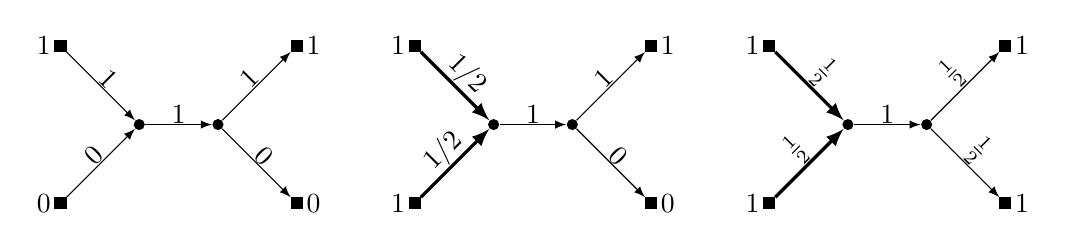
\begin{tikzpicture}[x=1cm,y=1cm,>=latex]
  \begin{scope}[xshift=0cm]
    \node[splitter] (s0) at (0,0) {};
    \node[splitter] (s1) at (1,0) {};
    \node[term] (i0) at (-1,1) {}; \draw (-1,1) node[anchor=east] {$1$};
    \node[term] (i1) at (-1,-1) {}; \draw (-1,-1) node[anchor=east] {$0$};
    \node[term] (o0) at (2,1) {}; \draw (2,1) node[anchor=west] {$1$};
    \node[term] (o1) at (2,-1) {}; \draw (2,-1) node[anchor=west] {$0$};
    \draw[->,fluid] (i0) -- (s0) node[midway,above=-3pt,sloped] {$1$};
    \draw[->,fluid] (i1) -- (s0) node[midway,above=-3pt,sloped] {$0$};
    \draw[->,fluid] (s0) -- (s1) node[midway,above=-3pt,sloped] {$1$};
    \draw[->,fluid] (s1) -- (o0) node[midway,above=-3pt,sloped] {$1$};
    \draw[->,fluid] (s1) -- (o1) node[midway,above=-3pt,sloped] {$0$};
  \end{scope}
  \begin{scope}[xshift=4.5cm]
    \node[splitter] (s0) at (0,0) {};
    \node[splitter] (s1) at (1,0) {};
    \node[term] (i0) at (-1,1) {}; \draw (-1,1) node[anchor=east] {$1$};
    \node[term] (i1) at (-1,-1) {}; \draw (-1,-1) node[anchor=east] {$1$};
    \node[term] (o0) at (2,1) {}; \draw (2,1) node[anchor=west] {$1$};
    \node[term] (o1) at (2,-1) {}; \draw (2,-1) node[anchor=west] {$0$};
    \draw[->,saturated] (i0) -- (s0) node[midway,above=-3pt,sloped] {$1/2$};
    \draw[->,saturated] (i1) -- (s0) node[midway,above=-3pt,sloped] {$1/2$};
    \draw[->,fluid] (s0) -- (s1) node[midway,above=-3pt,sloped] {$1$};
    \draw[->,fluid] (s1) -- (o0) node[midway,above=-3pt,sloped] {$1$};
    \draw[->,fluid] (s1) -- (o1) node[midway,above=-3pt,sloped] {$0$};
  \end{scope}
  \begin{scope}[xshift=9cm]
    \node[splitter] (s0) at (0,0) {};
    \node[splitter] (s1) at (1,0) {};
    \node[term] (i0) at (-1,1) {}; \draw (-1,1) node[anchor=east] {$1$};
    \node[term] (i1) at (-1,-1) {}; \draw (-1,-1) node[anchor=east] {$1$};
    \node[term] (o0) at (2,1) {}; \draw (2,1) node[anchor=west] {$1$};
    \node[term] (o1) at (2,-1) {}; \draw (2,-1) node[anchor=west] {$1$};
    \draw[->,saturated] (i0) -- (s0) node[midway,above=-3pt,sloped] {$\frac{1}{2}$};
    \draw[->,saturated] (i1) -- (s0) node[midway,above=-3pt,sloped] {$\frac{1}{2}$};
    \draw[->,fluid] (s0) -- (s1) node[midway,above=-3pt,sloped] {$1$};
    \draw[->,fluid] (s1) -- (o0) node[midway,above=-3pt,sloped] {$\frac{1}{2}$};
    \draw[->,fluid] (s1) -- (o1) node[midway,above=-3pt,sloped] {$\frac{1}{2}$};
  \end{scope}

\end{tikzpicture}

\end{document}